
\chapter{Основные понятия и обзор существующих алгоритмов}
\label{chapter1}

В этой главе введены термины и понятия, присутствующие в работе, произведен обзор существующих алгоритмов, затем сформулирована постановка задачи.

\section{Недоминирующая сортировка}

В данном разделе представлены основные понятия и определение недоминирующей сортировки. 

\subsection{Определение}

Для определения недоминирующей сортировки необходимо ввести отношение доминирования по Парето. Будем обозначать в данной работе $N$ {---} число точек, $M$ {---} число критериев точек.

\emph{Определение.} В $M$-мерном пространстве, точка $p = (p_1,...,p_M)$ доминирует по Парето точку $q = (q_1,...,q_M)$, обозначается как $p \prec q$, если для всех $1 \leq i \leq M$ выполняется неравенство $p_i\leq q_i$, и существует такое $j$, что $p_j < q_j$.

\emph{Определение.} Недоминирующая сортировка {---} это процедура назначения ранов точкам множества $S$ в многомерном пространстве $R^m$. Точки, которые не доминируются ни одной другой точкой, имеют ранг $0$. Остальные ранги назначаются следующим образом: точка имеет ранг $i + 1$, если максимальный ранг среди
доминирующих её точек равен $i$.

На Рисунке~\ref{nds} представлен пример недоминирующей сортировки для девяти точек в двумерном пространстве. Множество точек с одинаковым рангом называют \emph{фронтом} или \emph{слоем}. На рисунке изображено три фронта. 

\begin{figure}[!h]
\begin{center}
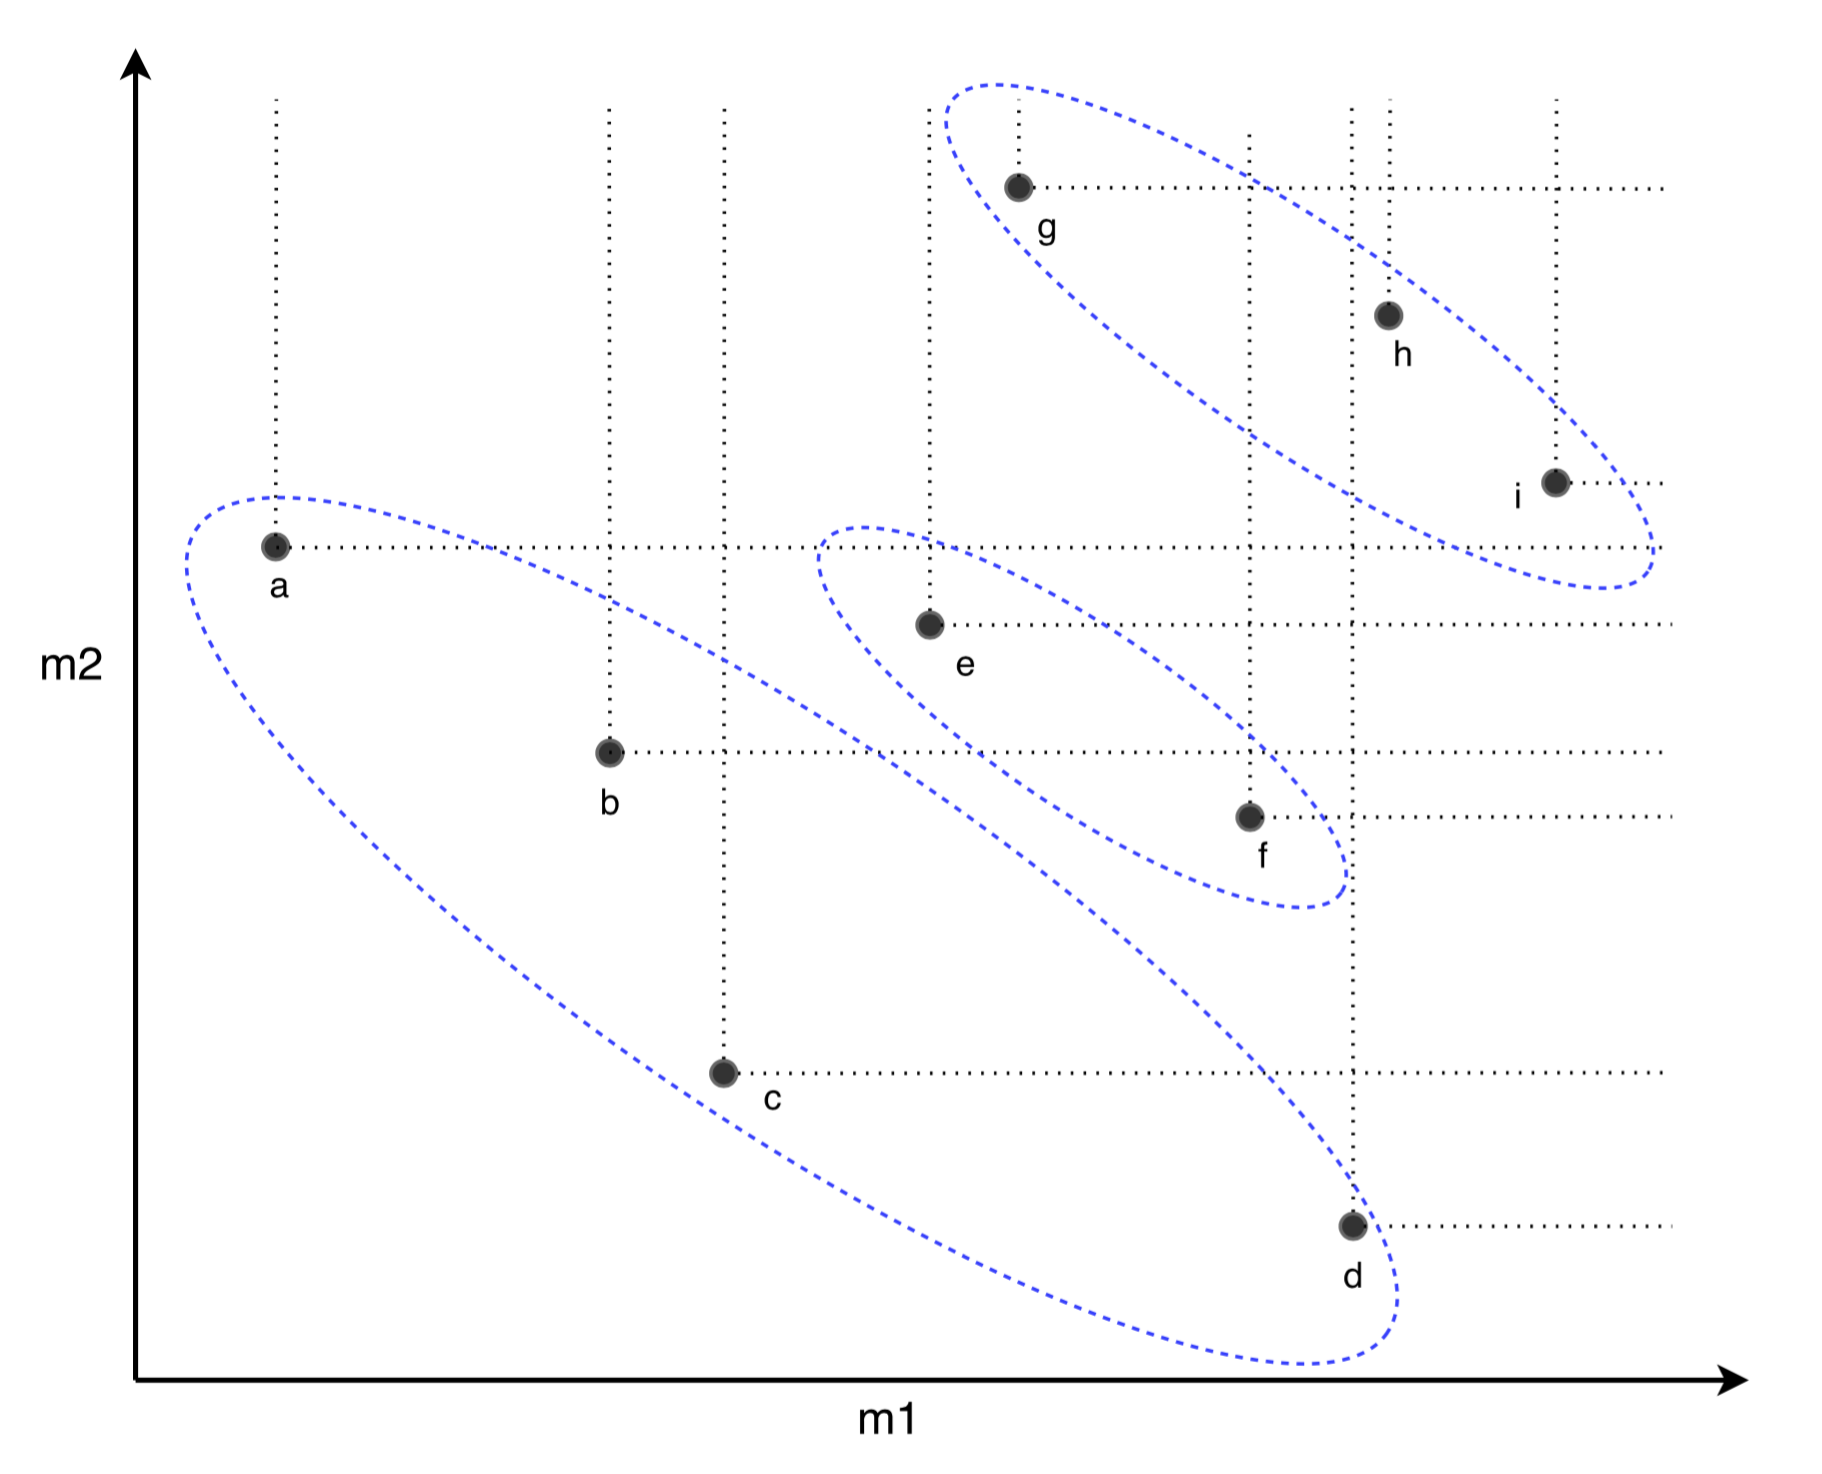
\includegraphics[width=0.8\textwidth]{pic/non_dominated_sort.png}
\caption{На рисунке представлен пример недоминирующей сортировки для точек $\{a,b,c,d,e,f,g,h,i\}$.
Точки $\{a,b,c,d\}$ имеют ранг $0$, $\{e,f\}$ {---} $1$, $\{g,h,i\}$ {---} $2$.}
\label{nds}
\end{center}
\end{figure}

\subsection{Область применения и актуальность}

Первоначально использование недоминирующей сортировки в эволюционных алгоритмах было предложено в~\cite{Srinivas}, она выполнялась за $O(N^3M)$. Позднее время работы было улучшено до $O(N^2M)$ в работе, в которой был представлен знаменитый алгоритм NSGA-II~\cite{NSGA-II}.

Эволюционные алгоритмы на каждой итерации генерируют множество потенциальных решений, надо отобрать набор лучших, для чего и требуется недоминирующая сортировка. 

Иногда подсчет каждого критерия для каждого решения занимает много времени, в этом случае время работы недоминирующей сортировки не имеет большого значения, так как асимптотика каждой итерации алгоритма зависит от вычисления критериев. Но гораздо чаще встречаются задачи, в которых подсчет каждого критерия занимает значительно меньше времени, чем необходимо для недоминирующей сортировки. Именно в таких случаях ускорение времени работы недоминирующей сортировки ускорит время выполнения каждой итерации алгоритма, а следовательно и время выполнения всего алгоритма.

Помимо фундаментального стремления к разработке эффективных алгоритмов, исследование, приведенное в данной работе, было мотивировано очень важной практической задачей: многокритериальной задачей оптимизации управления топливом, быстрое решение которой необходимо в ходе функционирования ядерного реактора~\cite{Schlunz}. Эта задача является сложной задачей оптимизации ряда противоречащих друг другу критериев, таких как мощность, получаемая от реактора, количество нейтронов, вылетающих из реактора и т. д. В 1995 году размер объектов для сортировки достигал $10^5$, сейчас он увеличился до $10^6$.

В настоящее время существуют много разных алгоритмов недоминирующей сортировки, но каждый из них имеет свои слабые стороны. Это означает, что есть возможность создать новый гибридный алгоритм, который будет совмещать в себе два других алгоритма, время работы которого будет лучше, как в теории, так и на практике.

\section{Анализ существующих алгоритмов}

В данном разделе рассмотрим историю развития алгоритмов недоминирующей сортировки. Особое внимание будет уделено самым эффективным алгоритмам, которые применяются для создания гибрида в данной работе.

\subsection{Наивные алгоритмы}

Наивный алгоритм недоминирующей сортировки перебирает все пары точек и сравнивает их по всем критериям. Точки, которые не доминируются ни одной другой точкой, получают ранг $0$ и исключаются из рассмотрения. Далее данная процедура повторяется, причем на каждом новом шаге присваивается новое значение ранга, на единицу больше, чем на предыдущем шаге. Время работы наивного алгоритма $O(MN^3)$, где $N$ {---} это число точек, а $M$ {---} размерность пространства, так как сравнение всех пар точек по $M$ критериям займет $O(MN^2)$, а всего шагов алгоритма будет не больше максимального числа рангов {---} $N$.

В работе Кунга и др.~\cite{Kung} предлагается алгоритм сортировки точек по слоям. То есть алгоритм недоминирующей сортировки следующий: сначала определяется минимальный слой, найденным точкам присваивается ранг $0$, и они исключаются из рассмотрения. Далее определяется минимальный слой на оставшихся точках, этим точкам присваивается ранг $1$. Процесс выполняется до тех пор, пока имеются точки, которым не присвоен ранг. Вычислительная сложностью поиска одного слоя равна $O(N log^{M-1} N)$. Описанная процедура в худшем случае выполняется за $O(N^2 log^{M-1} N)$, если максимальный найденный ранг равен $O(N)$.

Также существует много других алгоритмов, асимптотика которых равна $O(MN^2)$, например, алгоритм ENS Жанга и др.~\cite{Zhang}.

\subsection{Алгоритмы семейства <<Разделяй и Властвуй>>}

Йенсен~\cite{Jensen} впервые предложил алгоритм недоминирующей сортировки с вычислительной сложностью $O(N log^{M-1} N)$. Однако корректность и оценка сложности алгоритма доказывалась в предположении, что никакие две точки не имеют совпадающие значения ни в какой размерности. Так как часто алгоритмы оптимизации работают с дискретными критериями, совпадение разных решений по одному критерию {---} часто встречающееся событие. Устранить указанный недостаток оказалось достаточно трудной задачей — первой успешной попыткой сделать это, насколько известно автору, является работа Фортена и др.~\cite{Forton}. Исправленный (или, согласно работе, «обобщенный») алгоритм представлен в работе~\cite{Jensen}, он корректно работает во всех случаях, и во многих случаях его время работы составляет $O(N log^{M-1} N)$, но для худшего случая доказана асимптотика только $O(N^2M)$. Наконец, в работе Буздалова и др.~\cite{Buzdalov} предложены модификации алгоритма из работы~\cite{Jensen}, которые позволили доказать оценку $O(N log^{M-1} N)$ в худшем случае, не нарушая корректности работы алгоритма.

В данной работе базовым алгоритмом для создания гибрида будет алгоритм Буздалова и др., поэтому опишем его подробнее. Основная идея алгоритма {---} принцип <<разделяй и властвуй>. Исходное множество делится на три подмножества по медиане по последнему критерию: первое множество содержит элементы, которые по последнему критерию меньше медианы, второе {---} равных, третье {---} больших. Далее алгоритм рекурсивно запускается на каждом подмножестве, при этом по возможности уменьшая количество значимых для сравнения критериев. На рисунке~\ref{fast_pic} схематически изображена идея алгоритма Буздалова на основе метода <<разделяй и властвуй>>.

\begin{figure}[!h]
\begin{center}
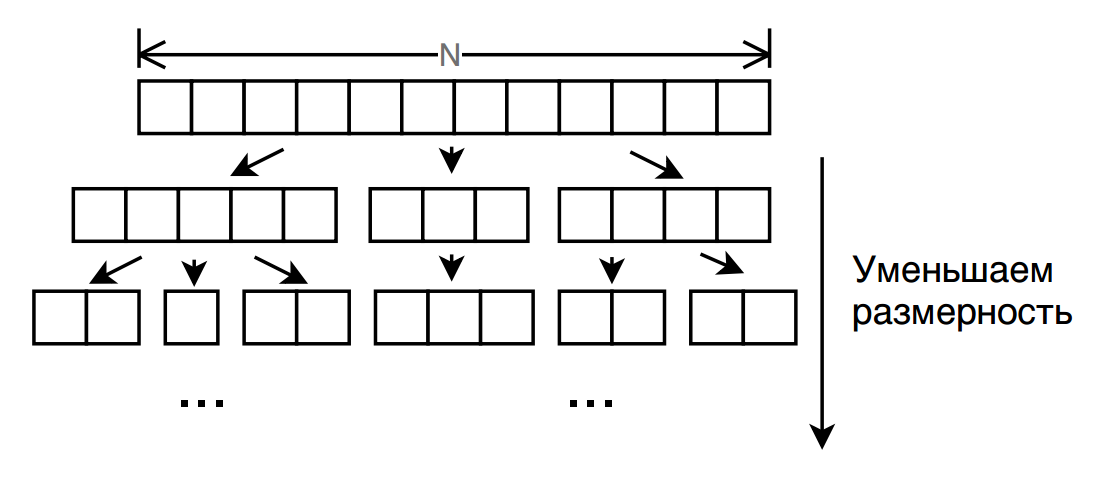
\includegraphics[width=10cm]{pic/fast_pic.png}
\caption{Идея алгоритма Буздалова на основе метода <<разделяй и властвуй>>.}
\label{fast_pic}
\end{center}
\end{figure}

Рассмотрим некоторые процедуры, использующиеся в алгоритме Буздалова, необходимые для понимания итогового гибридного алгоритма. Основными из них являются процедуры $HelperA$ и $HelperB$. Первая процедура $DivideConquerSorting$ представляет из себя основной алгоритм недоминирующей сортировки на множестве $S$, которое в качестве аргумента приходит на вход. Данная процедура сравнивает точки только по первым $k$ критериям. При запуске недоминирующей сортировки все точки инициализируются рангом $0$, и запускается процедура $HelperA$ c аргументами $S$ и $M$, где $M$ {---} это размерность пространства.

%TODO определиться с названием множества P или S 

Процедура $HelperA$ на размерности два запускает алгоритм на основе сканирующей прямой с асимптотической сложностью $O(n \log n)$.

В остальных случаях процедура $HelperA$ находит медианное значение $q$ и, используя это значение, разбивает множество точек на три подмножества $P_L$, $P_M$, $P_R$ с помощью процедуры $Split$. Множества определяются как $P_L = \{p \in P | p_j < q\}$, $P_M = \{p \in P | p_j = q\}$ и $P_R = \{p \in P | p_j > q\}$. После такого разбиения ни одна точка из множества правее не может доминировать ни одну точку из множества левее. Используя это свойство, мы можем найти ранги для множества $P_L$ независимо от других, затем обновить ранги множества $P_M$ на основе ранов множества $P_L$, далее независимо найти ранги множества $P_M$, используя уже поставленные на предыдущем шаге ранги. Аналогичный процесс продолжается для третьего множества $P_R$.

Псевдокод основной процедуры недоминирующей сортировки $DivideConquerSorting$ и процедуры $HelperA$ представлен на Листинге~\ref{nd-helper-a}.

\begin{algorithm}
\begin{algorithmic}[1]
\Procedure{DivideConquerSorting}{S, M}
    \State {$\textsc{Инициализация рангов}$ $0$}
    \State $HeplperA(S, M)$
\EndProcedure
\Procedure{HelperA}{S, k}
    \If{$|S| <= 1$} \Return
    \ElsIf{$|S| = 2$}
        \State {$\textsc{Сравнить точки по первым k критериям}$}
    \ElsIf{$k = 2$}
        \State {$\textsc{Алгоритм на основе сканирующей прямой}$}
    \Else
        \State{$q \gets \textsc{Median}(\{s_m|s \in S\})$}
        \State{$P_L, P_M, P_R \gets \textsc{Split}(S, m, q)$}
        \State{\textsc{HelperA}($P_L$, $k$)}
        \State{\textsc{HelperB}($P_L$, $P_M$, $k - 1$)}
        \State{\textsc{HelperA}($P_M$, $k - 1$)}
        \State{\textsc{HelperB}($P_L \cup P_M$, $P_R$, $k - 1$)}
        \State{\textsc{HelperA}($P_R$, $k$)}
    \EndIf
\EndProcedure
\end{algorithmic}
\caption{Основная процедура \textsc{$DivideConquerSorting$} и процедура \textsc{$HelperA$}, которая назначает ранги точкам из $S$ по первым $k$ критериям.}
\label{nd-helper-a}
\end{algorithm}

Следующая процедура $HelperB$ запускается между рекурсивными запусками $HelperA$ на двух подмножествах $L$ и $R$. Задача этой процедуры {---} обновить ранги второго множества $R$ на основе первого $L$, для дальнейшего запуска на втором множестве процедуры $HelperA$. Данная процедура также использует принцип <<разделяй и властвуй>> и при расстановке рангов разбивает множества на более мелкие и запускается на них рекурсивно.

На Листинге~\ref{nd-helper-b} представлен псевдокод процедуры $HelperB$.

\begin{algorithm}
\begin{algorithmic}[1]
\Procedure{HelperB}{L, R, k}
    \If{$|L| <= 1$ or $R <= 1$} \Return
        \State {$\textsc{Сравнить все пары точек по первым k критериям}$}
    \ElsIf{$k = 2$}
        \State {$\textsc{Алгоритм на основе сканирующей прямой}$}
    \ElsIf{$\min\{l_k | l \in L\} \le \max\{h_k | h \in H\}$}
        \State{$q \gets \textsc{Median}(\{p_m|p \in L \cup H\})$}
        \State{$L_L, L_M, L_R \gets \textsc{Split}(L, m, q)$}
        \State{$R_L, R_M, R_R \gets \textsc{Split}(R, m, q)$}
        \State{\textsc{HelperB}($L_L$, $R_L$, $k$)}
        \State{\textsc{HelperB}($L_R$, $R_R$, $k$)}
        \State{\textsc{HelperB}($L_L \cup L_M$, $R_M \cup R_R$, $k - 1$)}
    \EndIf
\EndProcedure
\end{algorithmic}
\caption{Процедура \textsc{$HelperB$}, которая обновляет ранги точек из $R$ на основе множества точек $L$ по первым $k$ критериям.}
\label{nd-helper-b}
\end{algorithm}

Асимптотическое время выполнения алгоритма сортировки на основе сканирующей прямой $O(n \log n)$, где $n$ {---} размер множества точек. Используя этот факт и то, что $max(|P_L|, |P_R|) \le 1/2 \cdot |P|$ и $max(|L_L| + |R_L|, |L_R| + |R_R|) \le 1/2 \cdot(|L| + |R|)$, далее можно использовать мастер-теорему~\cite{Cormen} для решения рекуррентного соотношения и доказать, что асимптотическое время работы алгоритма равно $O(|P| \cdot (\log|P|)^{M-1})$ в худшем случае.

\subsection{Алгоритм Роя и др.}

Некоторый интерес для рассмотрения в качестве кандидата для создания гибрида представляет алгоритм Роя $Best~Order~Sort~(BOS)$~\cite{Roy}, вычислительная сложность которого $O(MN \log N+MN^2)$. В лучшем случае алгоритм работает за $O(MN \log N)$, что лучше, чем время работы алгоритма, предложенного Буздаловым и др, но в худшем случае его асимптотика {---} $O(MN^2)$. 

Опишем кратко идею этого алгоритма, так как в данной работе была рассмотрена возможность создания гибридного алгоритма с использованием алгоритма Роя. Хотя она и не увенчалась успехом, но это исследование представляет некоторый научный интерес, так как показывает важность выбора алгоритмов при создании гибридного алгоритма. Более детальное описание алгоритма Роя можно найти в статье~\cite{Roy}.

Идея алгоритма в следующем: для каждой точки составим по каждому критерию множество, которое доминируется этой точкой. Получаем $M$ множеств для каждой точки. Далее для того, чтобы найти ранг точки $s$ достаточно рассмотреть только одно из $М$ множеств, соответствующих точке $s$. Назовем это множество $T$. Предположим, максимальный ранг точек из $T$ равен $r$, тогда точка $s$ будет иметь ранг $(r+1)$. Важным моментом является то, что любое множество из $M$ множеств может быть рассмотрено для поиска ранга $s$. Алгоритм $BOS$ находит для каждой точки минимальное возможное множество для этой цели. Чтобы это обеспечить, будем поддерживать множества $Q_1, Q_2, ..., Q_M$ для каждого критерия. Каждое $Q_i$ будет содержать отсортированный набор точек по критерию $i$. Далее будем определять ранги точек в следующем порядке: сначала для первой точки из множества $Q_1$, затем для первой точки из $Q_2$, так до множества по последнему критерию $Q_M$. Потом перейдем ко вторым точкам множеств и так далее. Если встретилась точка, ранг которой мы уже определили, пропускаем эту точку. На Рисунке~\ref{bos_descr} изображены $Q_1$ и $Q_2$ для некоторого множества двумерных точек. Стрелками показан порядок обхода точек. Процесс завершается как только все точки будут иметь ранг.

\begin{figure}
\begin{center}
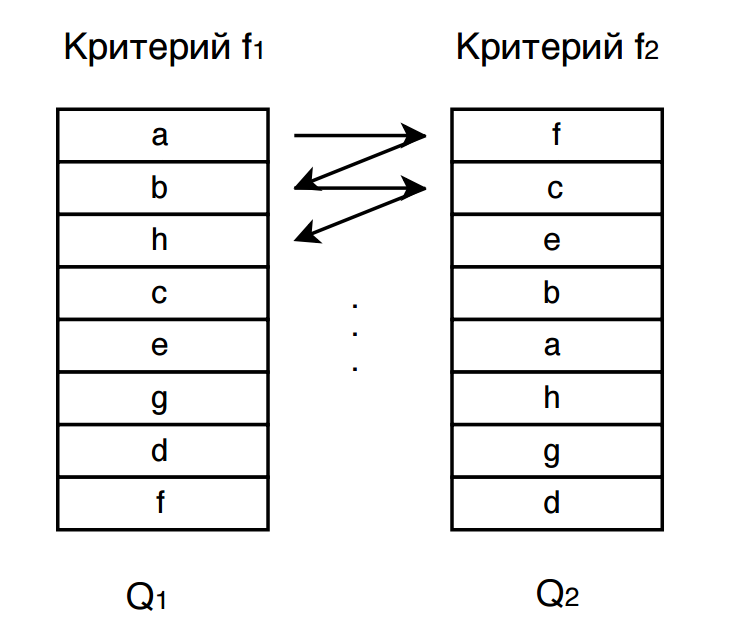
\includegraphics[width=9cm]{pic/bos_pic}
\caption{На рисунке представлены отсортированные списки по критерию $f_1$ и $f_2$. Точка $b$ будет сравниваться только с точкой $a$ и впоследствии ее ранг не будет меняться.}
\label{bos_descr}
\end{center}
\end{figure}

% TODO Переделать картинку, добавить текст
% Серым обозначены точки, для которых определяется ранг, остальные точки пропускаются {---} для них ранг был определен на предыдущих этапах.

Последним важным моментом в описании этого алгоритма является то, что определение ранга в каждом множестве происходит последовательным поиском по подмножествам одного ранга от минимального до максимального. То есть для определения ранга точки $s$, мы находим в соответствующем ей множестве $Q_i$ подмножество, соответствующее минимальному рангу, где ни одна точка не доминирует точку $s$. Если точки найденного подмножества имеют ранг $r$, то точке $s$ будет назначен ранг $r$. Это свойство назовем \emph{монотонностью}. Монотонность гарантирует, что ни одна точка из других подмножеств c большим рангом, не будет доминировать нашу точку $s$, и мы назначили ранг корректно. Благодаря монотонности определение ранга происходит быстро. А нарушение ее влечет значительное замедление. Впоследствии именно это станет основной причиной, почему создание эффективного гибридного алгоритма на основе алгоритма Роя и алгоритма Буздалова невозможна. 

\subsection{Алгоритм Густавссона и др.}

Большой интерес представляет алгоритм Густавссона и Соберфильдта ENS-NDT~\cite{Gustavsson}, который основан на применении $k$-$d$ деревьев ($k$-мерных деревьев). Его вычислительная сложность на случайно сгенерированных независимых точек равна $O(N^{1.43})$. Однако в худшем случае алгоритм работает за квадратичное время $O(MN^2)$.

Опишем основную идею этого алгоритма и приведем псевдокоды основных методов. Такое подробное описание необходимо в данной работе для понимания оптимизаций, модификаций алгоритма и для понимания итогового гибридного алгоритма. Более детальное описание можно найти в статье~\cite{Gustavsson}.

Алгоритм Густавссона и Сиберфильдта ENS-NDT относится к группе алгоритмов Efficient Non-dominated Sort(ENS). Еще одним представителем этой группы является алгоритм ENS-BS (Efficient Non-dominated Sort Binary Strategy), скорость работы которого сильно ухудшается с ростом количества точек. Алгоритм ENS-NDT справляется и с большим количеством точек, и с точками большой размерности в общем случае.

Алгоритм ENS-NDT использует недоминирующее дерево (NDTree). Недоминирующее дерево основано на корзиночных (bucket) $k$-$d$ деревьях. 

\emph{Определение.} Корзиночное $k$-$d$ дерево - это вид бинарного дерева, где хранятся точки $k$-мерного пространства. В узловых вершинах не содержится точек, в каждом узле происходит разделение множества точек на два подмножества по некоторому критерию: половина точек, имеющих большее значение критерия, отправляется в правого ребенка, остальные {---} в левого. Все точки содержатся в листьях. Размер множеств точек в листьях ограничен \emph{размером корзины (bucket size)}, который является параметром $k$-$d$ дерева. Если появляется необходимость добавить больше точек, вершина делится на две. Также глубина дерева ограничена параметром \emph{максимальной глубины дерева}. Если достигнута максимальная глубина дерева, параметр размера корзины игнорируется. 

Каждый уровень дерева ассоциирован с одной размерностью. Корневая вершина соответствует первому критерию, второй слой узлов соответствует второму критерию и так далее. Если родительский параметр ассоциирован с максимальной размерностью, слой наследников будет снова соответствовать первому критерию. 

При добавлении новой точки сначала производится спуск по дереву до соответствующего листа. Затем корзина листа пополняется, если размер корзины не превышен. В ином случае происходит создание двух вершин-наследников, в которые попадают точки согласно разделению по медиане по соответствующему родительской вершине критерию.

На рисунке~\ref{ndt_explanation} подставлена иллюстрация корзиночного $k$-$d$ дерева. Вершина $A$ ассоциирована с критерием $X$, вершины $B$ и $C$ ассоциирована с критерием $Y$, вершины $D$ и $E$ ассоциирована снова с критерием $X$. Размер корзины представленной на рисунке структуры равен трем.

\begin{figure}[!h]
\begin{center}
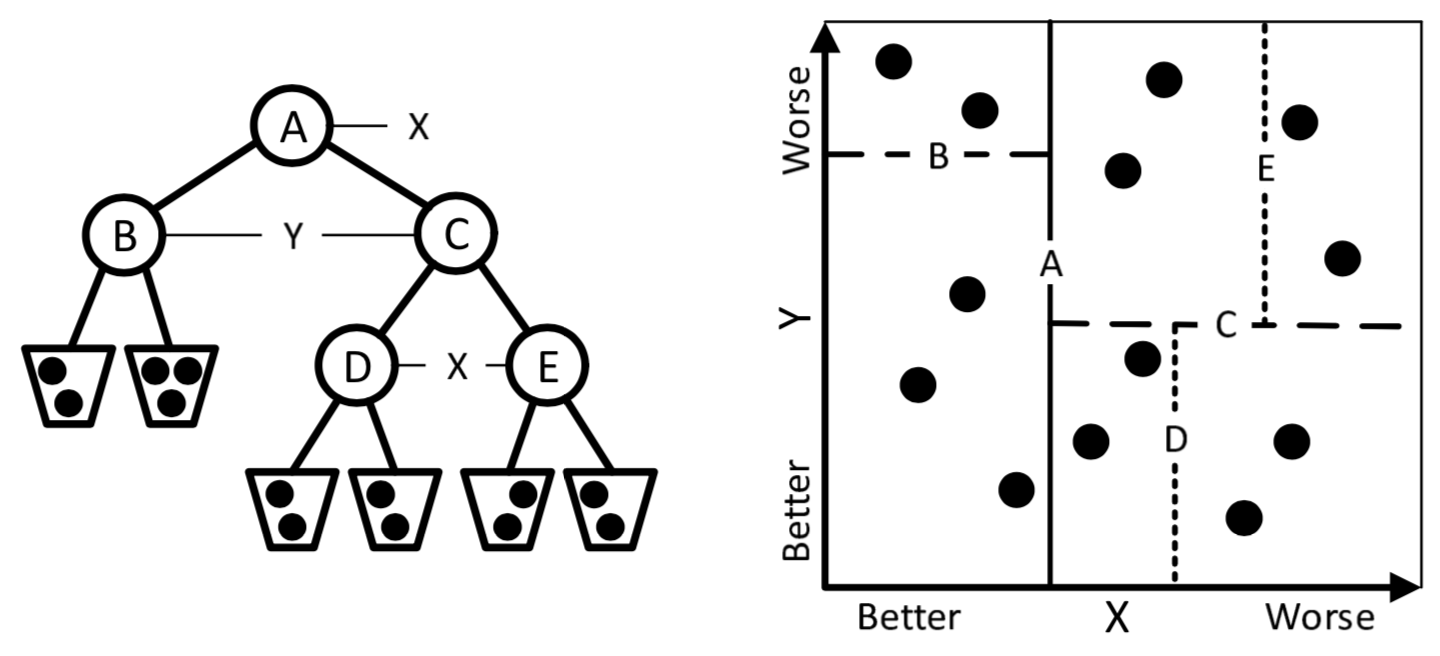
\includegraphics[width=0.8\textwidth]{pic/ndt_explanation.png}
\caption{Иллюстрация внутреннего устройства структуры корзиночного $k$-$d$ дерева. Слева изображена структура, справа точки на плоскости, по которым получена структура.}
\label{ndt_explanation}
\end{center}
\end{figure}

В алгоритме Густавссона для выполнения недоминирующей сортировки следует поддерживать отдельное дерево для каждого ранга. На Рисунке~\ref{ndtree_original} представлена схема структуры $k$-$d$ использующейся в недоминирующей сортировке.

\begin{figure}[!h]
\begin{center}
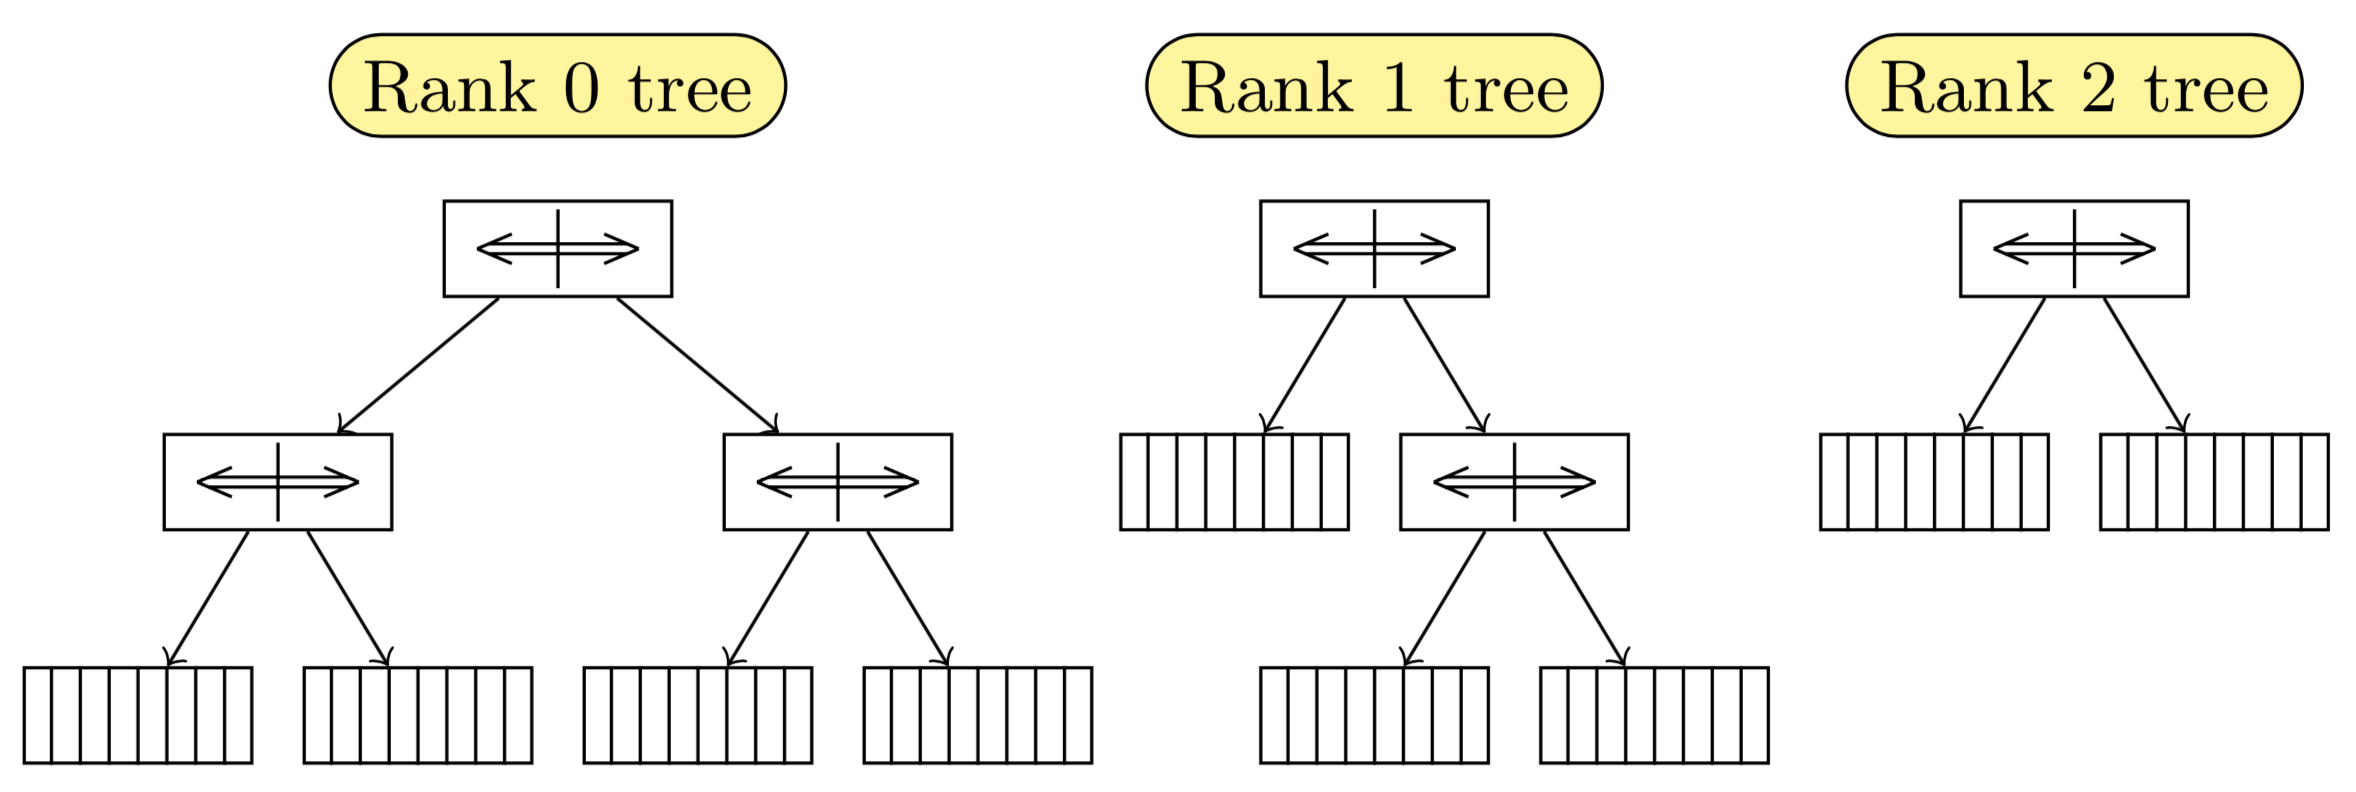
\includegraphics[width=0.8\textwidth]{pic/ndtree_original.png}
\caption{Структура деревьев для алгоритма ENS-NDT. Каждое дерево ассоциировано с отдельным рангом.}.
\label{ndtree_original}
\end{center}
\end{figure}

Недоминирующее дерево использует предподсчитанную $split$ структуру, где все возможные медианные значения преподсчитаны до того, как они потребуются. Отдельно уточним для избежания путаницы, что $split$ структура не имеет ничего общего с известной структурой данных, называемой $split$ деревьями. Предподсчет всех медиан заранее не используется в стандартной реализации корзиночного $k$-$d$ дерева, в котором обычно значения считаются в момент переполнения размера корзины в вершине. Это возможно сделать, потому что мы знаем множество точек для недоминирующей сортировки заранее. $Split$ структуру удобно хранить в виде $k$-$d$ дерева, похожего на финальное недоминирующее дерево. Основное преимущество использования $split$ структуры заключается в том, что недоминирующее дерево остается сбалансированным, что значительно улучшает производительность добавления вершин и определения ранга. 

Для выполнения недоминирующей сортировки следует выполнить следующие действия:
\begin{enumerate}
\item Создать $split$ структуру для всех точек.
\item Осуществить лексикографическую сортировку точек.
\item Перебирать точки в лексикографическом порядке.
    \begin{enumerate}
    \item Определить ранг.
    \item Добавить в соответствующее рангу дерево.
    \end{enumerate}
\end{enumerate}

На Листинге~\ref{procedure_end_ndt} представлен псевдокод основного метода недоминирующей сортировки, который принимает в качестве аргументов множество точек $P$, $M$ {---} размерность и $B$ {---} размер корзины. Для получения $split$ структуры используется функция $CreateSplits$, которая на вход получает множество точек, размер корзины и размерность $M-1$. Одна размерность игнорируется, так как ранее множество точек было лексикографически отсортировано. Лексикографическая сортировка выбрана еще потому, что она позволяет уменьшить число сравнений впоследствии.

Следующим шагом является создание множества $\mathcal{F}$ и $\mathcal{T}$ в Строках 4-6, $\mathcal{F}$ {---} это ранжированное множество точек, $\mathcal{T}$ {---} множество деревьев для каждого ранга, в каждом дереве ни одна точка не доминирует другую точку в том же дереве. Точка $P_1$ добавляется в оба множества с рангом один, так как ни одна другая точка не может доминировать первую в лексикографическом порядке точку. Главный цикл на Строке 8 определяет ранги точек и добавляет их в структуру.

\begin{algorithm}
\begin{algorithmic}[1]
\Procedure{ENS-NDT}{P, M, B}
    \State{$P \gets Sort(P, a^M \prec b^M, ..., a^1 \prec b^1)$}
    \State{$S \gets CreateSplits(P, M-1,B)$}
    \State{$\mathcal{F} \gets \{\{P_1\}\}$}
    \State{$\mathcal{T} \gets \{new NDTree(S, B)\}$}
    \State{$InsertIntoNDTree(\mathcal{T}_1, P_1)$}
    \State{$j \gets 1$}
    \For{$i = 2, ..., |P|$}
        \If{$P_{i-1} \neq P_{i}$}
            \State {$j \gets FrontIndexBinarySearch(\mathcal{T}, P_i)$}
            \If{$j > |\mathcal{T}|$}
                \State{$F_j \gets 0$}
                \State{$\mathcal{T}_j \gets new NDTree(S, B)$}
            \EndIf
            \State{$InsertIntoNDTree(\mathcal{T}_j, \mathcal{P}_i,)$}
        \EndIf
        \State{$\mathcal{F}_j \gets \mathcal{F}_j \cup {P_i} $}
    \EndFor
    \State{\Return {$\mathcal{F}$}}
\EndProcedure
\end{algorithmic}
\caption{Главная процедура алгоритма ENS-NDT.}
\label{procedure_end_ndt}
\end{algorithm}

% TODO Изменить ENS-NDT на $ENS$-$NDT$ ?
% TODO Изменить ENS-NDT-ONE на $ENS$-$NDT$-$ONE$ ?

Возможная реализация $CreateSplits$ приведена на Листинге~\ref{create_split}. Структура $NDSplit$ похожа на $NDTree$, но вместо точек она хранит медианные значения. Общий подход построения сбалансированных $k$-$d$ деревьев с помощью метода <<разделяй и властвую>> описан Бламом и др.~\cite{Blum}.

Вкратце опишем процедуру $CreateSplit$. Процедура принимает четыре аргумента: множество точек $P$, число критериев $M$, размер корзины $B$ и текущая глубина дерева $d$. При первом вызове процедуры $CreateSplit$ текущая глубина равна $0$. Далее значение текущей глубины дерева используется для выбора координаты в Строке 2, для которой происходит поиск медианного значения. Затем множество точек $P$ сортируется в Строке 3 по выбранному критерию, а переменной $m$ в Строке 4 присваивается значение медианы, как среднего значения в отсортированном множестве. Далее создается новая вершина дерева, и если множество не помещается в одну вершину по ограничению на размер корзины, то создается два наследника $Better$ и $Worse$. После чего происходит рекурсивный вызов процедуры $CreateSplits$ для обоих подмножеств с увеличенным значением глубины. Таким образом создается $split$ структура, которая возвращается в Строке 12. 

\begin{algorithm}
\begin{algorithmic}[1]
\Procedure{CreateSplit}{$P, M, B, d \gets 0$}
    \State{$o \gets 1 + (d \mod M)$}
    \State{$P \gets Sort(P, a^o \prec b^o)$}
    \State{$m \gets P_{1+\lfloor |P|/2 \rfloor}$}
    \State{$S \gets \{new NDSplit(o, m)\}$}
    \If{$|P|> B$}
        \State {$Better \gets \{P_i, i<1+\lfloor |P|/2 \rfloor\}$}
        \State {$Worse \gets \{P_i, i\geq1+\lfloor |P|/2 \rfloor\}$}
        \State {$S.BetterSplit \gets CreateSplit(Better, M, B, d+1)$}
        \State {$S.WorseSplit \gets CreateSplit(Worse, M, B, d+1)$}
    \EndIf
    \State{\Return S}
\EndProcedure
\end{algorithmic}
\caption{Пример реализации процедуры $CreatSplit$, которая вычисляет медианные значения для недоминирующего дерева.}
\label{create_split}
\end{algorithm}

Последней интересной для нас функцией является функция определения ранга точки $FrontIndexBinarySearch$, представленная на Листинге~\ref{rank_binary_search}. Эта процедура бинарным поиском определяет минимальное дерево в структуре $\mathcal{T}$, где ни одна точка не доминировала бы рассматриваемую. 

\begin{algorithm}
\begin{algorithmic}[1]
\Procedure{FrontIndexBinarySearch}{$\mathcal{T}, s$}
    \State{$i \gets 1$}
    \State{$j \gets |\mathcal{T}| + 1$}
    \While {$i \neq j$}
        \State {$k \gets \lfloor i + (j-i) /2 \rfloor $}
        \If {$FromntDominates(\mathcal{T}_k, s)$}
            \State {$i \gets k + 1$}
        \Else
            \State {$j \gets k$}
        \EndIf    
    \EndWhile
    \State{\Return i}
\EndProcedure
\end{algorithmic}
\caption{Процедура определения ранга точки $s$.}
\label{rank_binary_search}
\end{algorithm}

Подробное описание алгоритма ENS-NDT необходимо для понимания дальнейших модификаций и самого гибридного алгоритма.

\section{Недостатки существующих алгоритмов}

Все описанные выше алгоритмы имеют разные преимущества и недостатки. Алгоритм Буздалова <<разделяй и властвуй>> имеет хорошую асимптотику, даже на самых плохих входных данных. Однако алгоритм сильно замедляется с ростом размерности задачи $M$. 

Алгоритм Роя, имеет интересную идею и показал хорошие результаты на практике. Однако теоретическое время его работы пока не исследовано. 

Алгоритм Густавссона имеет хорошую асимптотику на случайно распределенных независимых точках в гиперкубе, но имеет квадратичную асимптотику в описанном авторами плохом случае. 

\section{Постановка задачи}

Цель данной работы состоит в разработке нового гибридного алгоритма недоминирующей сортировки и разбивается на задачи:
\begin{enumerate}
	\item Выбрать наиболее подходящие для алгоритмы.
	\item Приспособить их для создания гибридного алгоритма.
	\item Реализовать гибридный алгоритм.
	\item Настроить гибридный алгоритм для эффективной работы.
\end{enumerate}
